\section{Kubernetes}

\begin{frame}{What is Kubernetes}
\begin{itemize}
\item Platform for managing containerized workloads and services
\begin{itemize}
\item Portable
\item Extensible
\item Open Source
\item Originally developed by Google for managing service deployment
\end{itemize}
\item Kubernetes (K8s)
\begin{itemize}
\item Kubernetes, from Greek, means helmsman or pilot
\item ``K8s'' comes from the 8 characters between the ``k'' and the ``s''
\end{itemize}
\end{itemize}
\end{frame}

\begin{frame}{Benefits of Kubernetes}
\begin{itemize}
\item Persistence
\item Load balancing
\item Self-healing
\item Automated rollouts and rollbacks
\item Resource optimization
\item Infrastructure as code
\end{itemize}
\end{frame}

\begin{frame}{Application Deployment Scenarios}
\centering
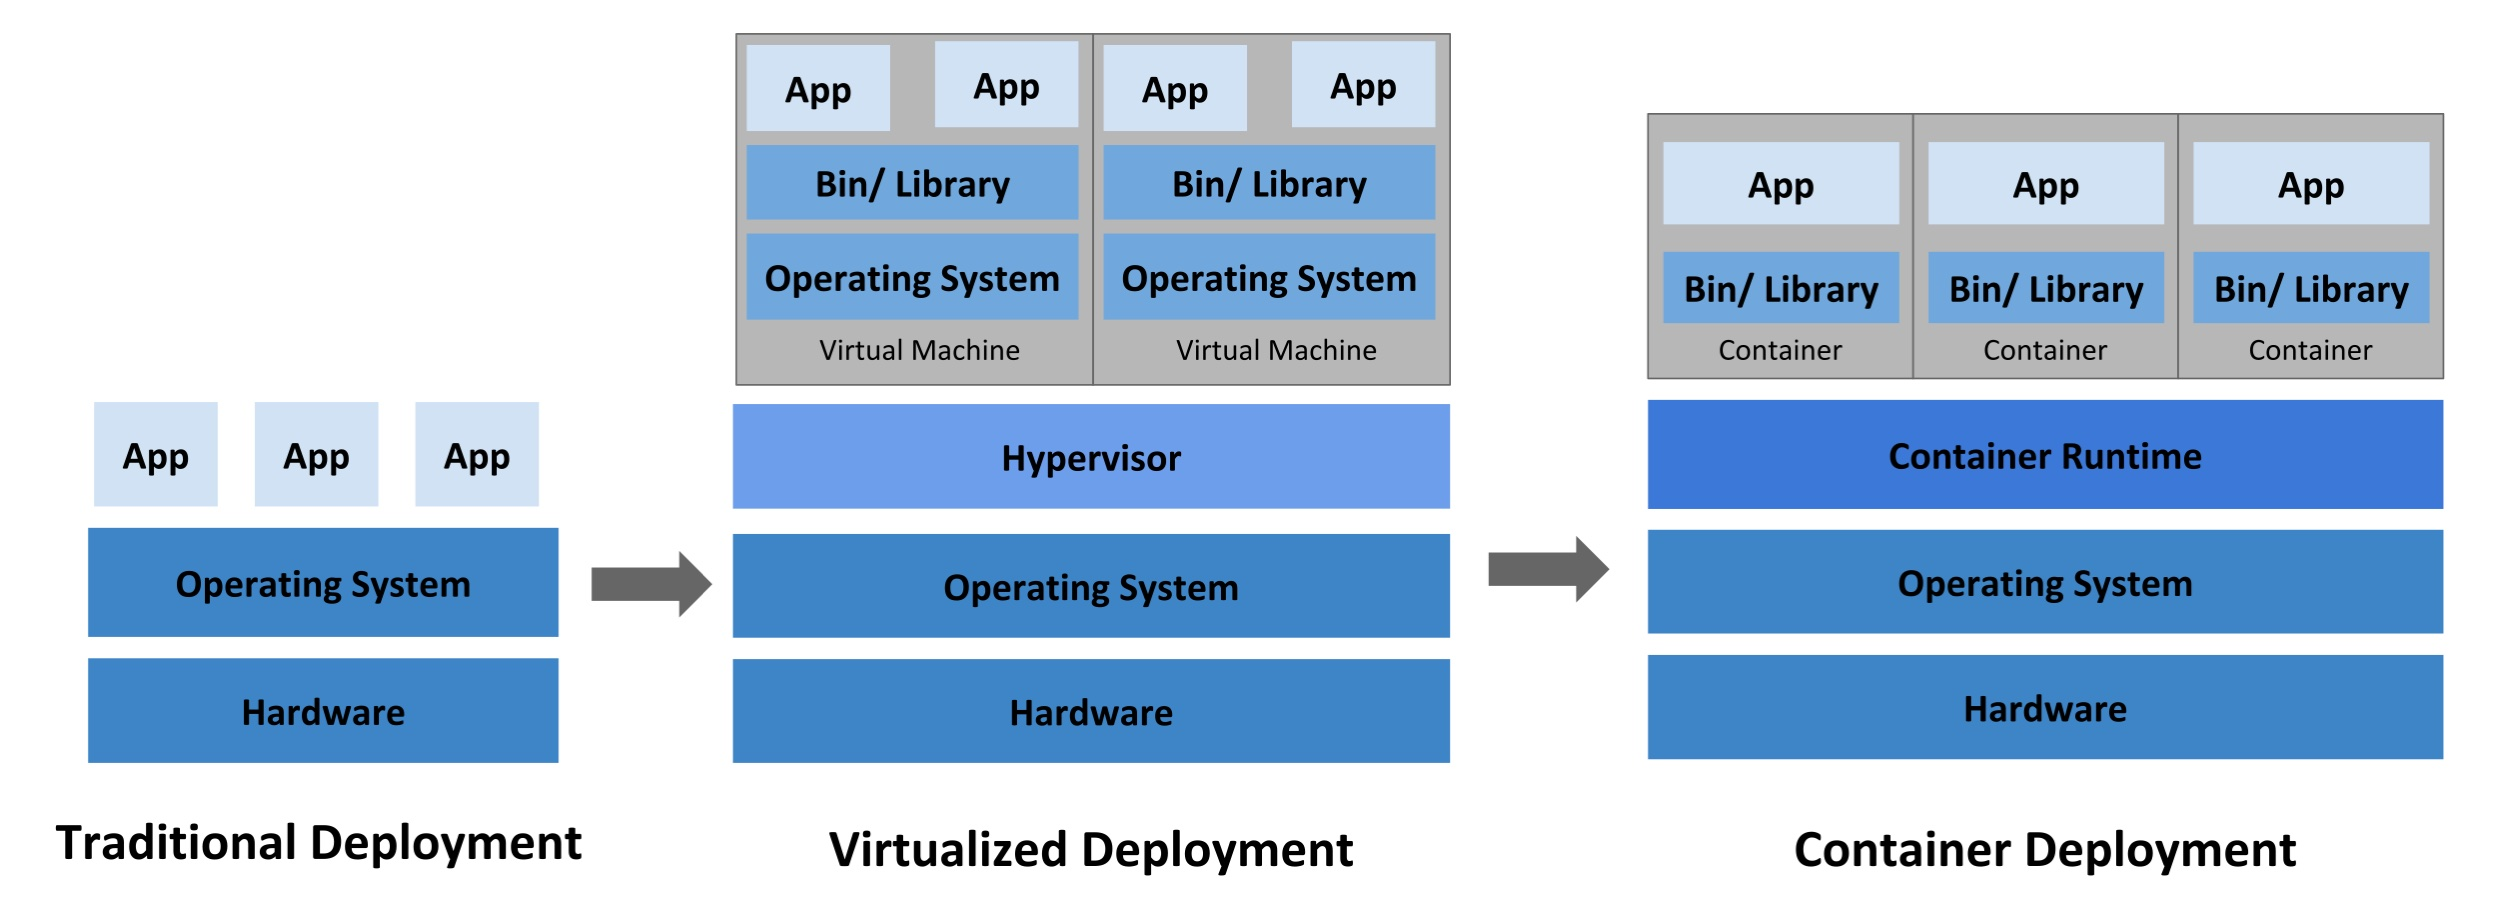
\includegraphics[height=0.7\textheight]{images/deployment_types.jpg}
\end{frame}

\begin{frame}{K8s Cluster Components}
\centering
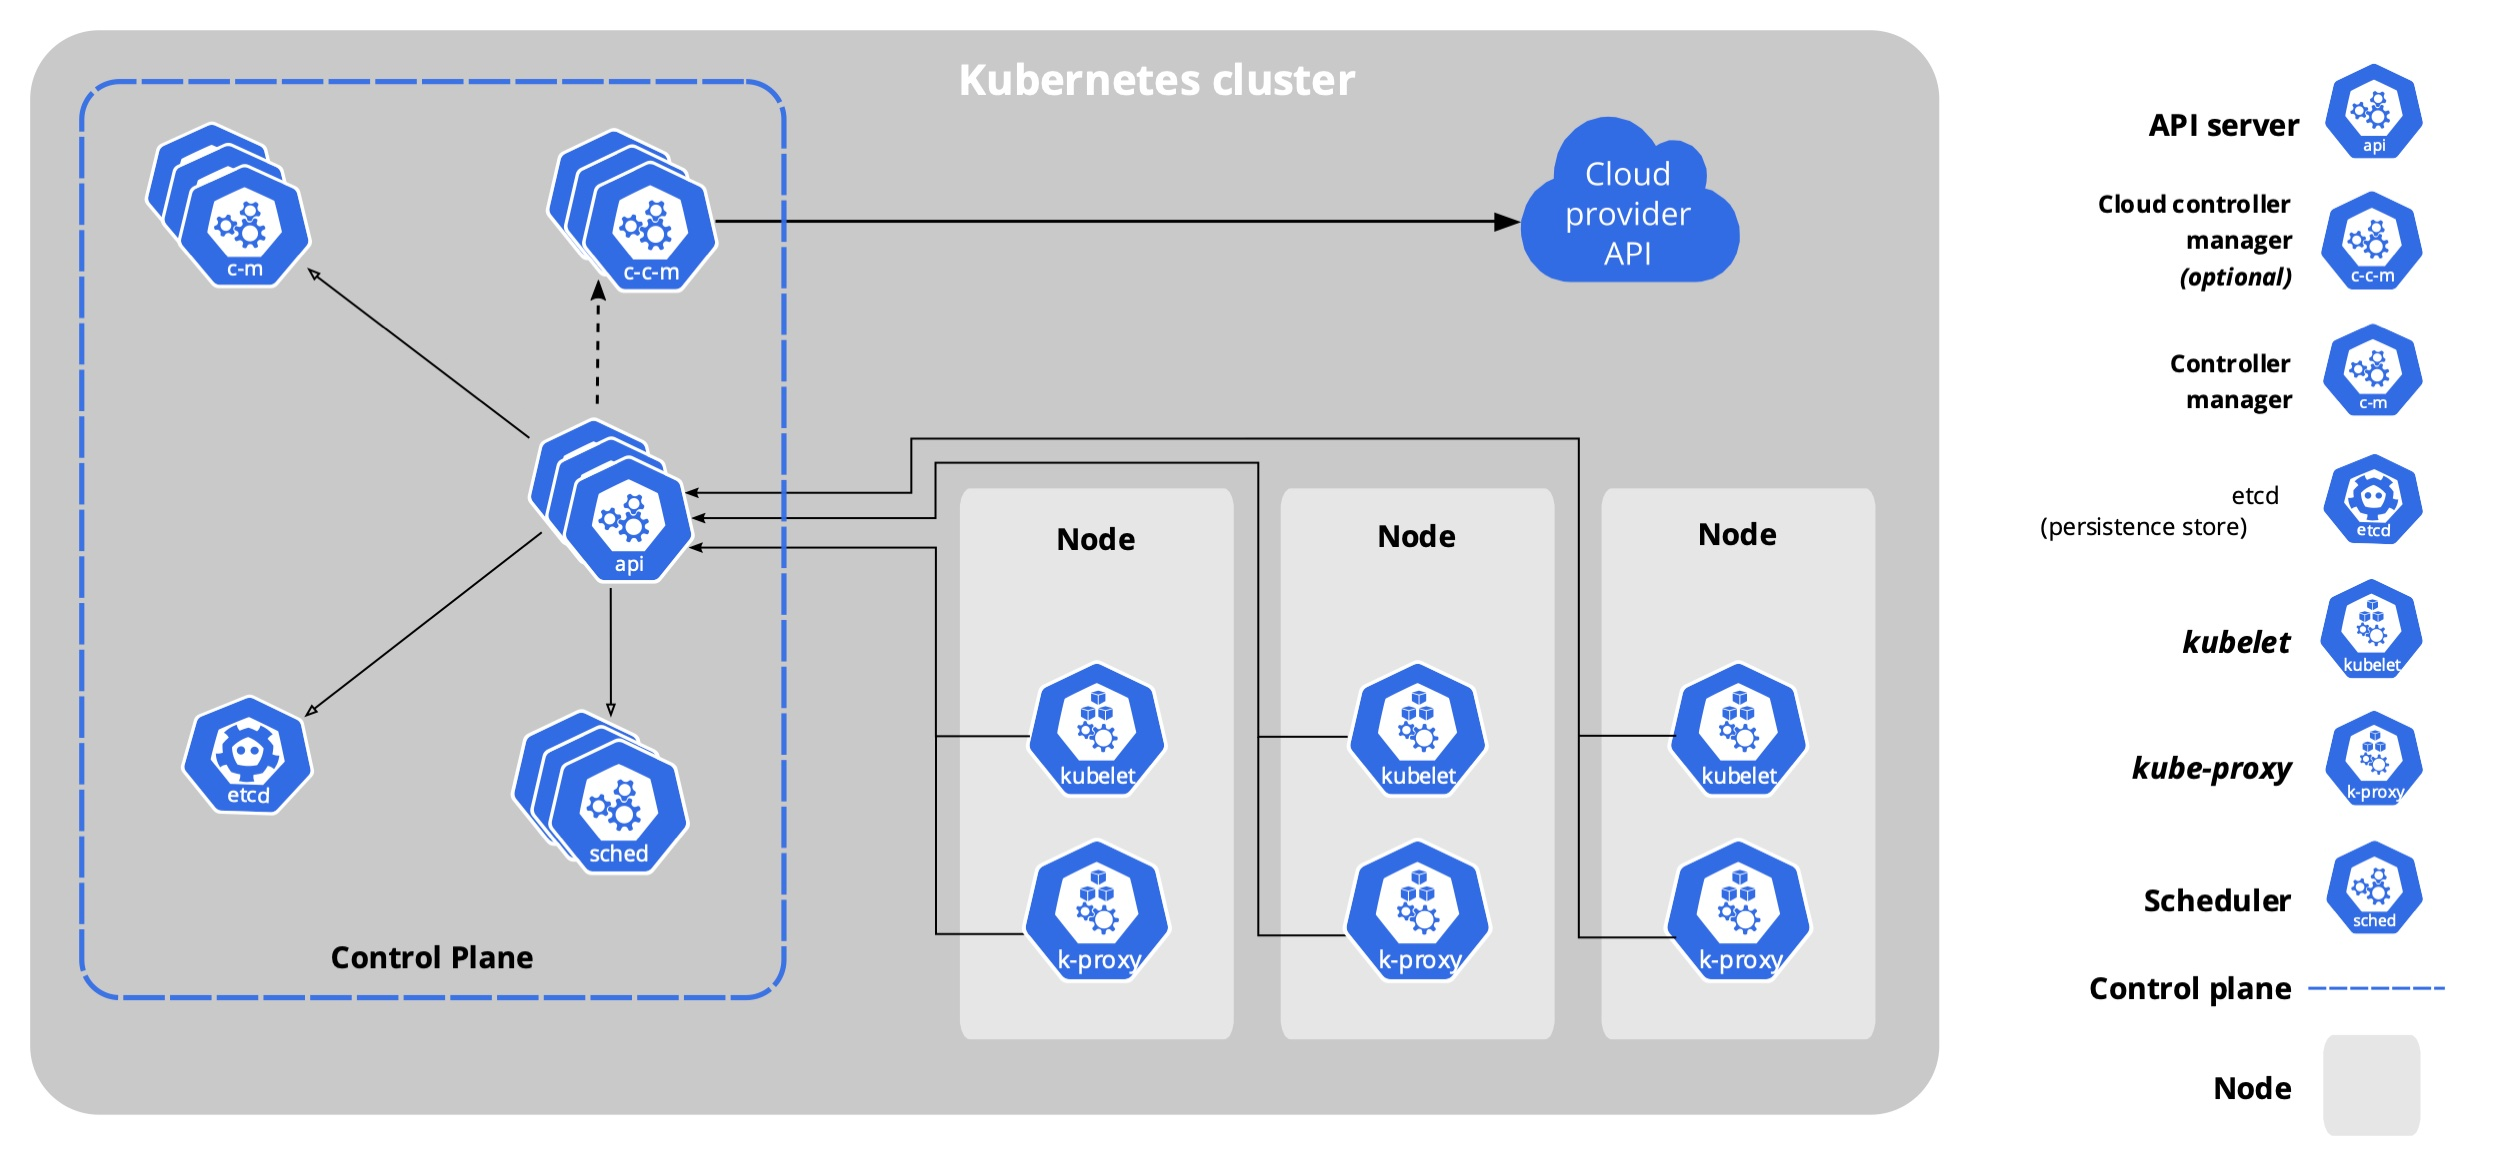
\includegraphics[height=0.7\textheight]{images/k8s_cluster.jpg}
\end{frame}

\begin{frame}{Kubernetes Distributions}
\scriptsize
\begin{columns}[c]
\begin{column}{0.5\textwidth}
\begin{itemize}
\item kubeadm
\item Minikube
\begin{itemize}
\item Local K8s clusters on macOS, Linux, and Windows
\item Commonly used for developing applications
\end{itemize}
\item K3s
\item GKE (Google Kubernetes Engine)
\item AKS (Microsoft Azure Kubernetes Services)
\item EKS (Amazon Elastic Kubernetes Service)
\item RKE (SUSE Rancher Kubernetes Engine)
\item Ubuntu
\begin{itemize}
\item Charmed Kubernetes
\item MicoK8s 
\end{itemize}
\end{itemize}
\end{column}
\begin{column}{0.5\textwidth}
\centering

\includegraphics[width=0.85\textwidth]{images/k8s_distributions.jpg}
\end{column}
\end{columns}
\end{frame}

\begin{frame}{Pods}
\begin{itemize}
\item Job definition
\begin{itemize}
\item One or more containers
\item Specification on how to run them
\end{itemize}
\item Shared resources
\begin{itemize}
\item Compute
\item Storage
\item Networking
\item Context
\begin{itemize}
\item Location and scheduling
\end{itemize}
\end{itemize}
\end{itemize}
\end{frame}

\begin{frame}{Types of Workloads}
\begin{description}
\item[Deployments] Manage changes to running Pods as specified rate
\item[ReplicaSet] Specify the number of available and identical Pods for high-availability
\item[StatefulSets] Deployment of Pods with a specific ordering, e.g. Pods with unique network IDs 
\item[DaemonSets] Every node gets a Pod, which dynamically changes as the cluster size changes
\item[Jobs] Batch scheduling of workloads (similar to Slurm Arrays, but with redundancy)
\item[Cronjobs] Scheduled workloads
\end{description}
\end{frame}

\begin{frame}{Pod Security}
\begin{itemize}
\item Specify the Pod level of isolation
\item Pod Security Standards
\begin{itemize}
\item Privileged (allows for privilege escalation)
\item Baseline (prevents privilege escalation)
\item Restricted (hardened security)
\begin{itemize}
\item Security-critical applications
\item Low-trust users
\end{itemize}
\end{itemize}
\item Levels of enforcement
\begin{itemize}
\item Enforce
\item Audit (log annotation)
\item Warn (user-facing warning)
\end{itemize}
\end{itemize}
\end{frame}

